\chapter{Schedulability Analysis Plugins Introduction}
\label{cha:schedulability-analysis-introduction}

\section{Generalities}


\subsection{Background}

Embedded control systems development is about producing systems or
sub-systems according to a set of specifications dictating their
required (physics) properties. The output of the design stage is a set
of models that describe the system at different levels of
abstraction. Properties and constraints are captured by mathematical
formalisms.

A typical design flow of embedded software (a v-shape process is
represented in Figure~\ref{fig:V-shaped-design-process.}) includes
(among others) two stages of fundamental importance. The first stage,
at the logical level, is the domain of application developers such as
control engineers or other domain experts and produces a model of the
software application providing a solution to the functional
requirements in terms of one or more block diagrams. Most commercial
design flows provide extensive support for this stage. Compliance
against functional requirements is typically validated by extensive
simulation and the risk of functional errors due to incorrect
implementation is reduced by tools for the automated translation of
the model (Real-Time Workshop Embedded Coder or TargetLink).

%
\begin{figure}
  \begin{center}
    \includegraphics[width=10cm]{images/vshape}
  \end{center}
  \caption{V-shaped design process.}
  \label{fig:V-shaped-design-process.}
\end{figure}


The second stage of the design process is at the architecture level,
where software engineers (real-time systems experts) map the
functions/components developed in the previous stage to real-time
threads, select the scheduler and the resource managers by exploiting
the services of a Real-Time Operating System (RTOS) and ultimately
check the correctness of the timing requirements upon the target (HW)
architecture. This design stage is transparent to software
functionality (only provides its implementation), but it is crucial to
achieve performance/cost trade-offs with the objective of providing
the best possible quality and the best possible accuracy to system
functions within the timing constraints and/or the performance target.


\subsection{Problem description}

Unfortunately, even in state-of-the-art processes, the above steps are
performed relying solely on the skills or the experience of project
developers. As a consequence, projects often suffer from design errors
that show up only after deployment with obvious economic losses. If
the software manufacturer detects timing errors or unsatisfactory
performance during the extensive testing period, a chain of
engineering changes is initiated that implies many iterations between
the logical and the architectural view, trading implementation
complexity for schedulability (or time performance) and tuning many
design parameters, including system resources and (when possible)
activation rates.

The separation of the design environments for functionality and for
time, together with the limited support (feedback) provided by the
existing tools make the process quite inefficient. Trial-and-error
iterations are often performed without a clear knowledge of what
should be modified and how.


\subsection{Innovating the architecture design}

Schedulability analysis theory bears the promise to fill in this gap,
since it enables formal validation of the timing behavior of
architecture-level solutions at the highest possible level in the
flow. To this purpose, timing properties and constraints should be
explicitly stated (by appropriate design annotations) and the
(hardware and software) resources available for the execution of the
application tasks and the resource allocation and scheduling policies
must be clearly stated in appropriate design environments.

We take inspiration from recent literature in the field of embedded
systems design, where a clear separation of concerns between
functional design and implementation choices is advocated and the use
of a shared set of abstractions allows for an efficient exchange of
information between the two activities. In this way, the functional
design remains independent from architectural choices and it does not
require an advance commitment to any specific implementation.


\section{The envisioned methodology: Architecture-level design}
\label{sec:envisioned-methodology}

\subsection{Introduction }

The distinctive aspect of schedulability analysis is a match between
the timing (or, in general, QoS) requirements of logical entities in
the logical layer and the corresponding QoS offers of an
implementation or architecture layer (Figure
\ref{fig:logical-phisical}) and consequently raises the fundamental
problem of mapping logical-level entities into architecture-level
entities \cite{OMG-PST02}.

The logical architecture\footnote{In the sequel, we shall use the
  adjective s{}``logical'' and {}``functional'' interchangeably.} (or
functional model) consists of a network of functional blocks or
components connected by means of communication variables and it is the
outcome of the control design phase. This network is typically a
straightforward derivation of the control schemes produced, for
example, using such CAD tools as Matlab/Simulink or ETAS ASCET-SD.
The concurrency description layer contains an implementation
description consisting of all the threads that are running in the
system and of the policies for managing resources (possibly
implemented in the operating system). Finally, the hardware layer
describes the hardware and its QoS features. The two bottom layers
collectively define the so-called physical architecture layer,
describing the mapping of the functional or logical design to a
particular real-time execution environment.

\begin{figure}
  \begin{center}
    \includegraphics[width=8cm]{images/logical-phisical.eps}
  \end{center}
  \caption{Schedulability analysis requires creating a correspondence
    between logical and physical architecture.}
  \label{fig:logical-phisical}
\end{figure}


The mapping stage consists of assigning each functional block to a
software thread and each communication variable to a communication
facility of the implementation (e.g. a task's private variable, a
protected shared variable, etc.). It also includes an appropriate
choice for such high level execution parameters as task activation
rates. In order to comply with the timing constraints, it is crucial
to perform appropriate choices for such real-time scheduling
parameters as, at this stage, task priorities and ceilings for
semaphores protecting shared resource (see the OSEK/VDX
specification). To this regard, a fundamental aid is offered by
schedulability analysis. This activity is performed right after
mapping (Figure \ref{fig:Schedulability-analysis}) to test the
correctness of a mapping hypotheses and to automatically synthesize
some of the real-time scheduling parameters.


\begin{figure}
\begin{center}
\includegraphics[width=10cm]{images/flow}
\par\end{center}
\caption{\label{fig:Schedulability-analysis}Schedulability analysis in
  the design flow}
\end{figure}


Several mapping-schedulability analysis iterations can be required
before coming up with a satisfactory design. In our envisioned
methodology such iterations are not \emph{blind-eyed} since
schedulability analysis does not simply provide a boolean answer on
the schedulability of the system, but it returns performance
information (i.e. response times) and sensitivity analysis. This
feedback drives mapping and/or architecture design changes but it can
also provide a measure of the resource (time) budgets that should be
accounted for in a possible functional redesign stage.


\subsection{Logical level design }
\label{sub:Logical-level-design}

At the logical level, most real-time systems feature a control and a
dataflow part. The dataflow part is often time-driven, since inputs
are sampled at regular intervals and it is suitable for an
implementation consisting mainly of periodic activities. In contrast,
the control-dominated functionality is highly asynchronous
(event-driven) and state-dependent.

The model of the system represents both parts with suitable
abstractions.  The syntax and the semantics of the modeling language
used by control engineers may vary, but in general, all models provide
a meta-representation of the design as a structure or network of
(functional) components connected via nets to each other's ports
(mechanisms to communicate between blocks, such as shared variables)
and communicating with each other using message (event)
abstractions. Messages may be asynchronous (signals) or synchronous
(call messages).

We provide a very simple and general metamodel (and a corresponding
syntax based on XML) for representing an abstraction of the functional
model where each component and event is annotated with timing
attributes and constraints, such as assumptions on the maximum rate of
arrival of events and on the worst case computation time of
components. This abstraction is suitable for specification of
architecture-level mapping and verification of timing properties.


\subsection{Software architecture design }
\label{sub:Software-architecture-design}

If the logical architecture primarily focuses on functional
requirements, the physical architecture level is where physical
concurrency, resource requirements and schedulability constraints are
expressed. At this level, the units of computation are the processes
or threads (or in general, tasks), executing concurrently in response
to environment stimuli or prompted by an internal clock. Tasks
cooperate by exchanging data and synchronization or activation signals
and compete for the use of shared resources (including the processor,
shared buffers, network links, etc.). Eventually, all logical entities
have to be mapped onto corresponding software architectural entities,
and the latter have to be mapped onto target hardware components in
the physical architecture level. This activity entails the selection
of an appropriate scheduling policy (for example, offered by a
real-time operating system), which must be clearly supported by
techniques for analyzing schedulability.

Our conceptual model uses the concepts of execution engine, scheduling
policy, resources, and schedulable resources to model the elements
of a physical architecture. An execution engine models the processing
resource and has a scheduling policy that determines how the tasks
will be scheduled. 


\subsection{Mapping}
\label{sub:Mapping}

The mapping process consists of establishing an \emph{implemented by}
or realization relationship between functional components and
architecture-level objects (such as tasks) and in the definition of a
binding or deployment relationship between threads and resources and
hardware components. The mapping relationship is constrained by the
specifications defined at both the logical and the architecture
levels, such as precedence and exclusion constraints among functional
blocks or timing constraints enforcing the activation rates of
software actions.

Mapping and binding decisions have crucial impact on the result of
timing analysis. Load balancing and local schedulability clearly
depend on binding decisions, when multiprocessor architectures are
considered.


\subsection{Schedulability Analysis}
\label{sub:Schedulability-Analysis}

Once the application functional model has been mapped on to a set of
real-time tasks, it is necessary to verify that all temporal
constraints are respected before actually implementing the system.

A real-time task is characterized by a period T (or minimum
interarrival time or maximum activation rate), by a relative deadline
D (i.e. the time computed from the activation by which each job must
complete) and by a worst-case execution time C. The goal of the
schedulability analysis is to check if all jobs can execute C units of
execution time between their activation time and their deadline.

For example, all OSEK-compliant OS provide the fixed priority
scheduling algorithm. For the fixed priority scheduling algorithm,
three different schedulability analysis can be performed: the
utilization-based test, the response time test and the hyperplane
test.

In case of detected timing failures, the Schedulability Analysis
returns feedback to the mapping in a form that allows the designer to
pinpoint the exact cause that lead to schedulability or timing errors
and give a range of actions as well as a measure of the entity of the
corrections that would make the design feasible.


\section{The Schedulability Analysis plugins}

The Schedulability Analysis plugins of \rtd\ aids the designer in
modeling, analyzing, and simulating the timing behavior of embedded
real-time systems. Being an open and extensible environment based on
XML and open standards (Java), \rtd\ can be easily integrated with
existing systems.

\begin{figure}
\begin{center}
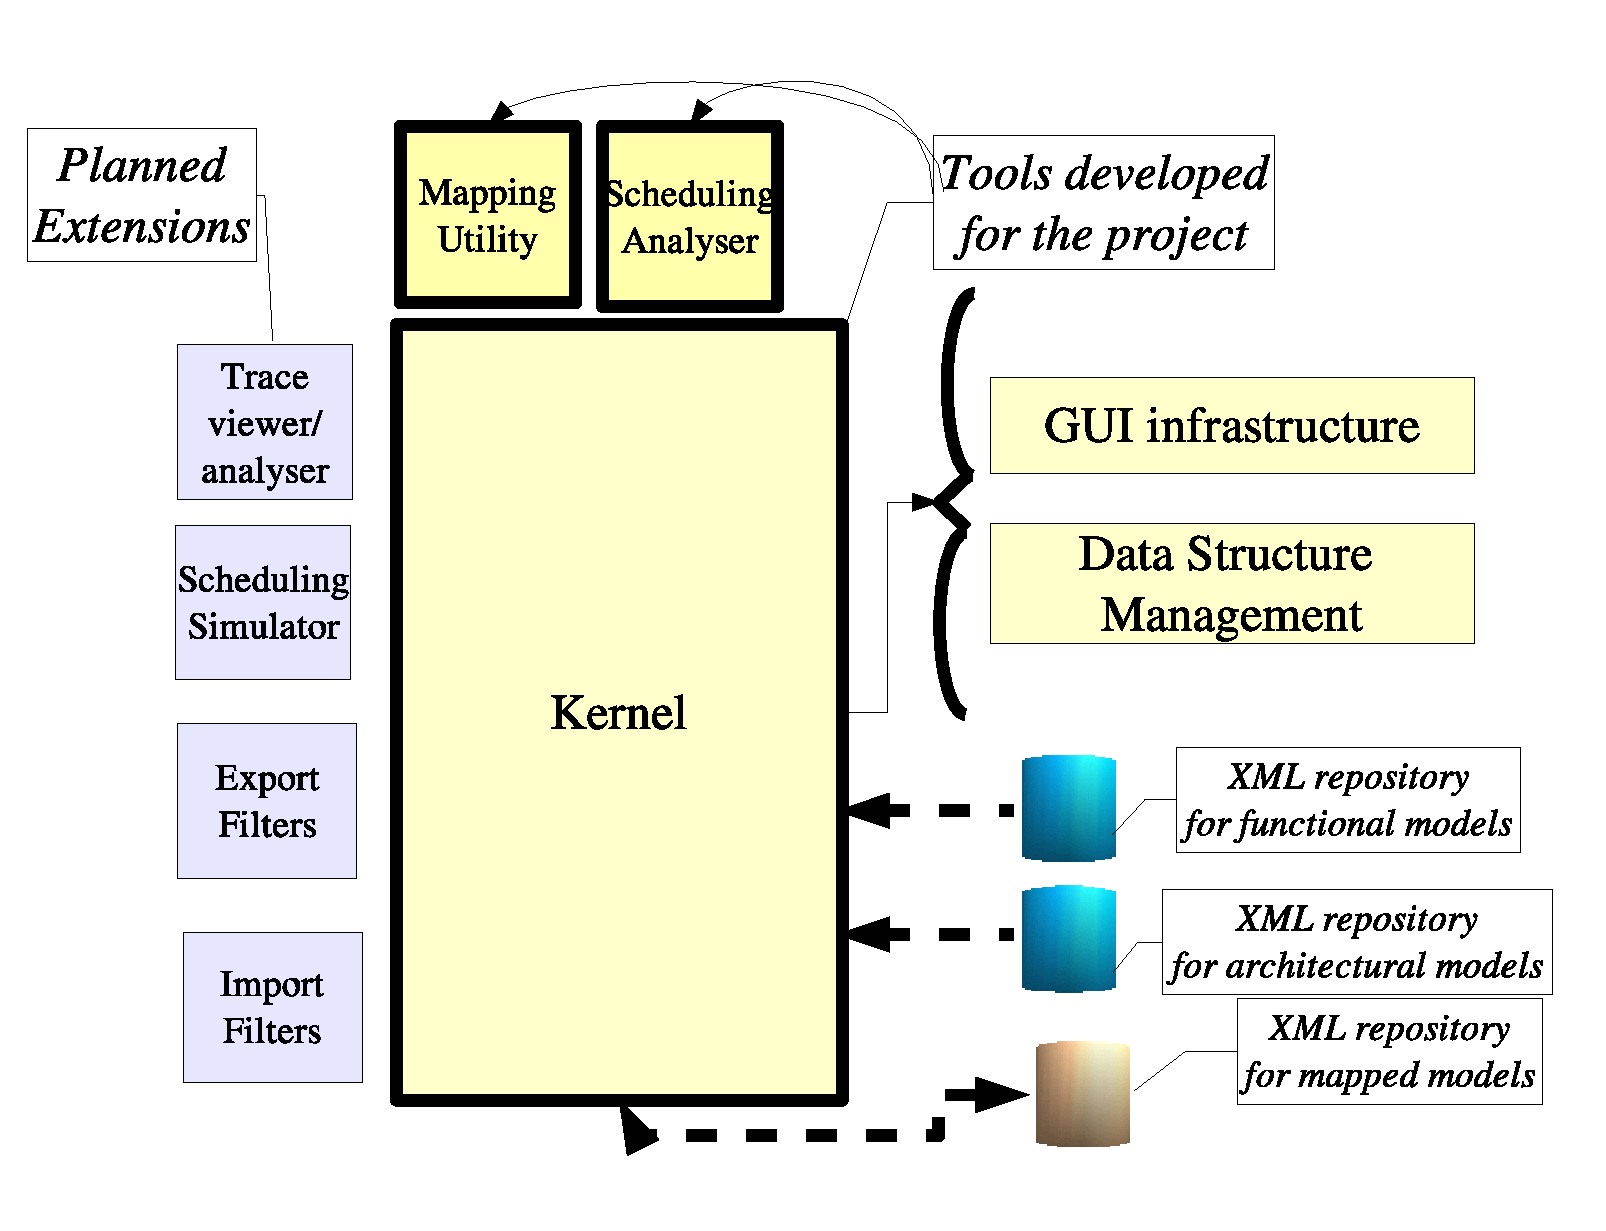
\includegraphics[width=10cm]{images/architecture}
\end{center}
\caption{\rtd\ architecture}
\label{fig:RTDruid-architecture}
\end{figure}


The \rtd\ schedulability plugins have a modular architecture shown in
Figure \ref{fig:RTDruid-architecture}.  Model information (i.e. for
both the functional and the architecture-level parts) is stored in an
internal repository and it is made available by means of an open
format based on XML. The tool set architecture is based on a kernel
module, providing management of internal data structure and basic
services for GUI and additional plugin modules.  Plugins exploit
kernel services in order to provide support to the design stages in a
completely independent way.

The modeling and mapping module provides general Graphics and Text
Diagrams to capture textual requirements, flowcharts, component and
deployment notation and other general purpose information. Design
teams can develop a representation of the embedded real-time system in
graphical or textual form and capture the interaction between
functional and architecture-level designs without disrupting the
existing development process. This is done by using a neutral
(XML-based) format and metamodel.  Both logical and architecture-level
modeling entities can be interactively defined within the context of
the tool or imported by translation from external models. XML-based
import/export utilities enable the transfer of information between our
tools and other tools supporting XML or text-based standards. Modeling
elements for logical and architecture-level abstractions mirror the
definitions given in the previous sections.

The \textbf{schedulability analyzer} plugin provides support for worst
case timing analysis. The module interacts with the other components
by exchanging design information in the form of back annotations
according to the schema of Figure
\ref{fig:schedulability-analysis-interactions}. The forward path of
Figure \ref{fig:schedulability-analysis-interactions} represents the
communication of the system model (as defined in the previous
sections) to the schedulability analysis tool. The inverse model
conversion provides an alternate option for using the results of the
schedulability analysis since it can produce its results in the same
XML files that are used to encode the design information. In
particular, it stores the values for the attributes (priority,
priority ceiling) that are synthesized based on the selected
scheduling policy and the schedulability results
themselves. Back-annotating the results into the same XML file that
represents the model of the system helps the designer in keeping all
the information related to the current iteration in the design flow
aligned and consistent.

\begin{figure}
\begin{center}
\includegraphics[width=10cm]{images/interoperability}
\end{center}
\caption{Interactions between the kernel module and the Schedulability analyzer.}
\label{fig:schedulability-analysis-interactions}
\end{figure}

% These are not implemented yet
%The \textbf{trace viewer/analyzer} provides support for estimating the
%execution time attributes of software components

%The \textbf{Scheduling simulator} enables an evaluation of the worst
%case response time of the threads needs to be supplemented by simulations
%of average as well as critical runs highlighting the expected time
%behavior of the system. 

%The \textbf{Export/import} filters automatically imports model diagrams
%from existing tools such as Simulink, ASCET or UML-based design frameworks. 

%The \textbf{Automatic code generation} features automates the production
%of functional as well as architecture-level code and debugging information
%in OSEK-compliant systems.


\subsection{Status of the Schedulability analysys plugin}

As shown in Figure \ref{fig:RTDruid-architecture}, the current version
of the tool offers a set of components that enables the user to
perform a schedulability analysis of the system under design. A
graphical GUI based on the Eclipse Project is available, which allows
the user to edit the input files, perform the schedulability analysis
and to visualize the related results.

The tool can be used as follows (see Figure \ref{fig:RTDflow}):

\begin{figure}
  \begin{center}
    \includegraphics[width=6.3cm]{images/RTDruid_flow3.eps}
  \end{center}
  \caption{Status of the Schedulability analysis plugin.}
  \label{fig:RTDflow}
\end{figure}

\begin{itemize}
\item The user is required to specify the system (inclusive of
  functional model, software architecture and mapping) by means of XML
  files, whose format is documented in Chapter
  \ref{cha:DTD-Input-file}. The input files can be edited with any
  text editor, or with the GUI. The system specification can be
  contained in one single XML files, or it can be split among many
  files. The tool will automatically merge all files in one single
  specification. The initial specification may also come from an input
  file expressed in OSEK OIL or AUTOSAR XML (typically in these cases
  the model must be augmented with execution time informations since
  these file formats are not meant for schedulability analysis but
  only for RTOS configuration).
\item Once the system has been specified, the user can run the tool in
  either batch mode or in graphical mode. To perform the operations in
  batch mode, the user must provide a Ant script file (see the Apache
  Ant project on the Apache web site). The script file features are
  described in Chapter \ref{cha:Script-File}. The tool invocation
  results into the execution of commands specified in the script file.
\item The results of schedulability analysis are then reported in an
  output file as well as in the \rtd\ Table view (if run from the
  graphical interface). It is possible to annotate the results in the
  same input files in a specific section.
\end{itemize}

